% Generated by Sphinx.
\def\sphinxdocclass{report}
\documentclass[letterpaper,10pt,brazil]{sphinxmanual}
\usepackage[utf8]{inputenc}
\DeclareUnicodeCharacter{00A0}{\nobreakspace}
\usepackage{cmap}
\usepackage[T1]{fontenc}
\usepackage{babel}
\usepackage{times}
\usepackage[Sonny]{fncychap}
\usepackage{longtable}
\usepackage{sphinx}
\usepackage{multirow}


\addto\captionsbrazil{\renewcommand{\figurename}{Fig. }}
\addto\captionsbrazil{\renewcommand{\tablename}{Tabela }}
\floatname{literal-block}{Listagem }



\title{Projeto Cuidando do Meu Bairro}
\date{23/12/2015}
\release{1.0}
\author{Cuidando}
\newcommand{\sphinxlogo}{}
\renewcommand{\releasename}{Versão}
\makeindex

\makeatletter
\def\PYG@reset{\let\PYG@it=\relax \let\PYG@bf=\relax%
    \let\PYG@ul=\relax \let\PYG@tc=\relax%
    \let\PYG@bc=\relax \let\PYG@ff=\relax}
\def\PYG@tok#1{\csname PYG@tok@#1\endcsname}
\def\PYG@toks#1+{\ifx\relax#1\empty\else%
    \PYG@tok{#1}\expandafter\PYG@toks\fi}
\def\PYG@do#1{\PYG@bc{\PYG@tc{\PYG@ul{%
    \PYG@it{\PYG@bf{\PYG@ff{#1}}}}}}}
\def\PYG#1#2{\PYG@reset\PYG@toks#1+\relax+\PYG@do{#2}}

\expandafter\def\csname PYG@tok@sx\endcsname{\def\PYG@tc##1{\textcolor[rgb]{0.78,0.36,0.04}{##1}}}
\expandafter\def\csname PYG@tok@ge\endcsname{\let\PYG@it=\textit}
\expandafter\def\csname PYG@tok@na\endcsname{\def\PYG@tc##1{\textcolor[rgb]{0.25,0.44,0.63}{##1}}}
\expandafter\def\csname PYG@tok@mo\endcsname{\def\PYG@tc##1{\textcolor[rgb]{0.13,0.50,0.31}{##1}}}
\expandafter\def\csname PYG@tok@mf\endcsname{\def\PYG@tc##1{\textcolor[rgb]{0.13,0.50,0.31}{##1}}}
\expandafter\def\csname PYG@tok@sc\endcsname{\def\PYG@tc##1{\textcolor[rgb]{0.25,0.44,0.63}{##1}}}
\expandafter\def\csname PYG@tok@il\endcsname{\def\PYG@tc##1{\textcolor[rgb]{0.13,0.50,0.31}{##1}}}
\expandafter\def\csname PYG@tok@err\endcsname{\def\PYG@bc##1{\setlength{\fboxsep}{0pt}\fcolorbox[rgb]{1.00,0.00,0.00}{1,1,1}{\strut ##1}}}
\expandafter\def\csname PYG@tok@gh\endcsname{\let\PYG@bf=\textbf\def\PYG@tc##1{\textcolor[rgb]{0.00,0.00,0.50}{##1}}}
\expandafter\def\csname PYG@tok@mb\endcsname{\def\PYG@tc##1{\textcolor[rgb]{0.13,0.50,0.31}{##1}}}
\expandafter\def\csname PYG@tok@nv\endcsname{\def\PYG@tc##1{\textcolor[rgb]{0.73,0.38,0.84}{##1}}}
\expandafter\def\csname PYG@tok@c\endcsname{\let\PYG@it=\textit\def\PYG@tc##1{\textcolor[rgb]{0.25,0.50,0.56}{##1}}}
\expandafter\def\csname PYG@tok@s1\endcsname{\def\PYG@tc##1{\textcolor[rgb]{0.25,0.44,0.63}{##1}}}
\expandafter\def\csname PYG@tok@nd\endcsname{\let\PYG@bf=\textbf\def\PYG@tc##1{\textcolor[rgb]{0.33,0.33,0.33}{##1}}}
\expandafter\def\csname PYG@tok@se\endcsname{\let\PYG@bf=\textbf\def\PYG@tc##1{\textcolor[rgb]{0.25,0.44,0.63}{##1}}}
\expandafter\def\csname PYG@tok@mi\endcsname{\def\PYG@tc##1{\textcolor[rgb]{0.13,0.50,0.31}{##1}}}
\expandafter\def\csname PYG@tok@kn\endcsname{\let\PYG@bf=\textbf\def\PYG@tc##1{\textcolor[rgb]{0.00,0.44,0.13}{##1}}}
\expandafter\def\csname PYG@tok@ni\endcsname{\let\PYG@bf=\textbf\def\PYG@tc##1{\textcolor[rgb]{0.84,0.33,0.22}{##1}}}
\expandafter\def\csname PYG@tok@gi\endcsname{\def\PYG@tc##1{\textcolor[rgb]{0.00,0.63,0.00}{##1}}}
\expandafter\def\csname PYG@tok@mh\endcsname{\def\PYG@tc##1{\textcolor[rgb]{0.13,0.50,0.31}{##1}}}
\expandafter\def\csname PYG@tok@nl\endcsname{\let\PYG@bf=\textbf\def\PYG@tc##1{\textcolor[rgb]{0.00,0.13,0.44}{##1}}}
\expandafter\def\csname PYG@tok@nn\endcsname{\let\PYG@bf=\textbf\def\PYG@tc##1{\textcolor[rgb]{0.05,0.52,0.71}{##1}}}
\expandafter\def\csname PYG@tok@gs\endcsname{\let\PYG@bf=\textbf}
\expandafter\def\csname PYG@tok@c1\endcsname{\let\PYG@it=\textit\def\PYG@tc##1{\textcolor[rgb]{0.25,0.50,0.56}{##1}}}
\expandafter\def\csname PYG@tok@w\endcsname{\def\PYG@tc##1{\textcolor[rgb]{0.73,0.73,0.73}{##1}}}
\expandafter\def\csname PYG@tok@bp\endcsname{\def\PYG@tc##1{\textcolor[rgb]{0.00,0.44,0.13}{##1}}}
\expandafter\def\csname PYG@tok@nf\endcsname{\def\PYG@tc##1{\textcolor[rgb]{0.02,0.16,0.49}{##1}}}
\expandafter\def\csname PYG@tok@sd\endcsname{\let\PYG@it=\textit\def\PYG@tc##1{\textcolor[rgb]{0.25,0.44,0.63}{##1}}}
\expandafter\def\csname PYG@tok@k\endcsname{\let\PYG@bf=\textbf\def\PYG@tc##1{\textcolor[rgb]{0.00,0.44,0.13}{##1}}}
\expandafter\def\csname PYG@tok@vi\endcsname{\def\PYG@tc##1{\textcolor[rgb]{0.73,0.38,0.84}{##1}}}
\expandafter\def\csname PYG@tok@gd\endcsname{\def\PYG@tc##1{\textcolor[rgb]{0.63,0.00,0.00}{##1}}}
\expandafter\def\csname PYG@tok@no\endcsname{\def\PYG@tc##1{\textcolor[rgb]{0.38,0.68,0.84}{##1}}}
\expandafter\def\csname PYG@tok@vc\endcsname{\def\PYG@tc##1{\textcolor[rgb]{0.73,0.38,0.84}{##1}}}
\expandafter\def\csname PYG@tok@vg\endcsname{\def\PYG@tc##1{\textcolor[rgb]{0.73,0.38,0.84}{##1}}}
\expandafter\def\csname PYG@tok@kt\endcsname{\def\PYG@tc##1{\textcolor[rgb]{0.56,0.13,0.00}{##1}}}
\expandafter\def\csname PYG@tok@gp\endcsname{\let\PYG@bf=\textbf\def\PYG@tc##1{\textcolor[rgb]{0.78,0.36,0.04}{##1}}}
\expandafter\def\csname PYG@tok@kp\endcsname{\def\PYG@tc##1{\textcolor[rgb]{0.00,0.44,0.13}{##1}}}
\expandafter\def\csname PYG@tok@cm\endcsname{\let\PYG@it=\textit\def\PYG@tc##1{\textcolor[rgb]{0.25,0.50,0.56}{##1}}}
\expandafter\def\csname PYG@tok@ss\endcsname{\def\PYG@tc##1{\textcolor[rgb]{0.32,0.47,0.09}{##1}}}
\expandafter\def\csname PYG@tok@go\endcsname{\def\PYG@tc##1{\textcolor[rgb]{0.20,0.20,0.20}{##1}}}
\expandafter\def\csname PYG@tok@cs\endcsname{\def\PYG@tc##1{\textcolor[rgb]{0.25,0.50,0.56}{##1}}\def\PYG@bc##1{\setlength{\fboxsep}{0pt}\colorbox[rgb]{1.00,0.94,0.94}{\strut ##1}}}
\expandafter\def\csname PYG@tok@nc\endcsname{\let\PYG@bf=\textbf\def\PYG@tc##1{\textcolor[rgb]{0.05,0.52,0.71}{##1}}}
\expandafter\def\csname PYG@tok@o\endcsname{\def\PYG@tc##1{\textcolor[rgb]{0.40,0.40,0.40}{##1}}}
\expandafter\def\csname PYG@tok@si\endcsname{\let\PYG@it=\textit\def\PYG@tc##1{\textcolor[rgb]{0.44,0.63,0.82}{##1}}}
\expandafter\def\csname PYG@tok@gt\endcsname{\def\PYG@tc##1{\textcolor[rgb]{0.00,0.27,0.87}{##1}}}
\expandafter\def\csname PYG@tok@sh\endcsname{\def\PYG@tc##1{\textcolor[rgb]{0.25,0.44,0.63}{##1}}}
\expandafter\def\csname PYG@tok@nt\endcsname{\let\PYG@bf=\textbf\def\PYG@tc##1{\textcolor[rgb]{0.02,0.16,0.45}{##1}}}
\expandafter\def\csname PYG@tok@kd\endcsname{\let\PYG@bf=\textbf\def\PYG@tc##1{\textcolor[rgb]{0.00,0.44,0.13}{##1}}}
\expandafter\def\csname PYG@tok@ne\endcsname{\def\PYG@tc##1{\textcolor[rgb]{0.00,0.44,0.13}{##1}}}
\expandafter\def\csname PYG@tok@gr\endcsname{\def\PYG@tc##1{\textcolor[rgb]{1.00,0.00,0.00}{##1}}}
\expandafter\def\csname PYG@tok@gu\endcsname{\let\PYG@bf=\textbf\def\PYG@tc##1{\textcolor[rgb]{0.50,0.00,0.50}{##1}}}
\expandafter\def\csname PYG@tok@nb\endcsname{\def\PYG@tc##1{\textcolor[rgb]{0.00,0.44,0.13}{##1}}}
\expandafter\def\csname PYG@tok@ow\endcsname{\let\PYG@bf=\textbf\def\PYG@tc##1{\textcolor[rgb]{0.00,0.44,0.13}{##1}}}
\expandafter\def\csname PYG@tok@s2\endcsname{\def\PYG@tc##1{\textcolor[rgb]{0.25,0.44,0.63}{##1}}}
\expandafter\def\csname PYG@tok@sb\endcsname{\def\PYG@tc##1{\textcolor[rgb]{0.25,0.44,0.63}{##1}}}
\expandafter\def\csname PYG@tok@kc\endcsname{\let\PYG@bf=\textbf\def\PYG@tc##1{\textcolor[rgb]{0.00,0.44,0.13}{##1}}}
\expandafter\def\csname PYG@tok@sr\endcsname{\def\PYG@tc##1{\textcolor[rgb]{0.14,0.33,0.53}{##1}}}
\expandafter\def\csname PYG@tok@cp\endcsname{\def\PYG@tc##1{\textcolor[rgb]{0.00,0.44,0.13}{##1}}}
\expandafter\def\csname PYG@tok@kr\endcsname{\let\PYG@bf=\textbf\def\PYG@tc##1{\textcolor[rgb]{0.00,0.44,0.13}{##1}}}
\expandafter\def\csname PYG@tok@s\endcsname{\def\PYG@tc##1{\textcolor[rgb]{0.25,0.44,0.63}{##1}}}
\expandafter\def\csname PYG@tok@m\endcsname{\def\PYG@tc##1{\textcolor[rgb]{0.13,0.50,0.31}{##1}}}

\def\PYGZbs{\char`\\}
\def\PYGZus{\char`\_}
\def\PYGZob{\char`\{}
\def\PYGZcb{\char`\}}
\def\PYGZca{\char`\^}
\def\PYGZam{\char`\&}
\def\PYGZlt{\char`\<}
\def\PYGZgt{\char`\>}
\def\PYGZsh{\char`\#}
\def\PYGZpc{\char`\%}
\def\PYGZdl{\char`\$}
\def\PYGZhy{\char`\-}
\def\PYGZsq{\char`\'}
\def\PYGZdq{\char`\"}
\def\PYGZti{\char`\~}
% for compatibility with earlier versions
\def\PYGZat{@}
\def\PYGZlb{[}
\def\PYGZrb{]}
\makeatother

\renewcommand\PYGZsq{\textquotesingle}

\begin{document}

\maketitle
\tableofcontents
\phantomsection\label{index::doc}


Versão 1.0 - dezembro de 2015.

Projeto \emph{Cuidando do Meu Bairro}: abertura e geolocalização do orçamento municipal.

\textbf{Acesso}:
\begin{itemize}
\item {} 
Portal e implantação para o município de São Paulo em  \href{http://cuidando.vc}{Cuidando.vc}.

\item {} 
Fontes de dados orçamentários nos \href{http://demo.gastosabertos.org}{webservices do projeto GastosAbertos.org}.

\end{itemize}

\textbf{Códigos-fonte} (repositórios \href{https://pt.wikipedia.org/wiki/Git}{git}):
\begin{itemize}
\item {} 
Site:
\href{https://github.com/okfn-brasil/cuidando2}{okfn-brasil/cuidando2}

\item {} 
Módulos de dados orçamentários:

\item {} 
Fontes dos engines e extratores:
\href{https://github.com/okfn-brasil/gastos\_abertos}{okfn-brasil/gastos\_abertos},
\href{https://github.com/okfn-brasil/teaser.gastosabertos.org}{teaser.gastosabertos.org}.

\item {} 
Dados e documentação:
\href{https://github.com/okfn-brasil/gastos\_abertos\_dados}{okfn-brasil/gastos\_abertos\_dados},
\href{https://github.com/okfn-brasil/documents/blob/master/gastos\_abertos}{okfn-brasil/documents/gastos\_abertos}.

\item {} 
Autenticação de usuários:
\href{https://github.com/okfn-brasil/viralata}{okfn-brasil/viralata}

\item {} 
Comunicação dos usuários:
\href{https://github.com/okfn-brasil/tagarela}{okfn-brasil/tagarela}

\item {} 
Intermediação do eSIC:
\href{https://github.com/okfn-brasil/esiclivre}{okfn-brasil/esiclivre}

\end{itemize}

\textbf{Documentação}:
\begin{itemize}
\item {} 
Tutoriais na \href{https://pt.wikiversity.org/wiki/Projeto\_Cuidando\_do\_Meu\_Bairro}{Wikiversity-Português, Projeto Cuidando do Meu
Bairro}.

\item {} 
Instruções para o desenvolvedor:
\href{https://github.com/okfn-brasil/cuidando2-doc}{okfn-brasil/cuidando2-doc}.

\item {} 
Administração do projeto:
\href{http://wiki.okfn.org/Open\_Knowledge\_Brasil/Gastos\_Abertos}{wiki.okfn.org}.

\end{itemize}


\chapter{Histórico e versões}
\label{index:cuidando-do-meu-bairro}\label{index:historico-e-versoes}
Este projeto teve origem no \href{http://cuidando.org.br}{Cuidando do Meu Bairro de
2013}, que buscava mapear a execução do
orçamento municipal de São Paulo, não só em regiões, mas também
colocando um ponto no mapa para cada despesa. Por isso o presente
projeto foi apelidado de \textbf{Cuidando2}: uma nova interface, novos
recursos e melhoras nos dados gerados pelo software.

Como os \href{http://orcamento.prefeitura.sp.gov.br/orcamento/execucao.html}{dados obtidos da
prefeitura}
não têm as coordenadas geográficas de cada despesa (no máximo algumas
tem a região a que se destinam), o ponto de partida são os endereços nos
textos das descrições das despesas, que por sua vez podem ser submetidos
à \href{https://en.wikipedia.org/wiki/Geocoding}{geocodificação} em
ferramentas adequadas.

A extração dos endereços a partir do texto é obtida através de \href{https://pt.wikipedia.org/wiki/Express\%C3\%A3o\_regular}{expressões regulares}. A geocodificação desses endereços é realizada pelas \href{https://en.wikipedia.org/wiki/Application\_programming\_interface}{API}s
\href{http://wiki.openstreetmap.org/wiki/Nominatim}{OpenStreetMap-Nomination}
e \href{https://developers.google.com/maps/documentation/geocoding/intro}{Google-geocoding}.
Esse processo não é perfeito, acumula erros tanto da fase de extração
como da fase de geocodificação, de modo que muitas despesas não são
mapeadas, ou acabam exibidas no local errado. No Cuidando2 o processo
foi aperfeiçoado para reduzir a taxa de erros.


\chapter{Arquitetura}
\label{index:arquitetura}
Buscando ampliar a chance de reuso do código desenvolvido e permitir um nível
maior de interação com outros aplicativos, o projeto seguiu uma arquitetura de
micro serviços. Ou seja, ao invés de ter um único código monolítico que
implementasse todas as funcionalidades desejadas, elas foram distribuídas em
pequenos módulos, cada um com uma funcionalidade específica:

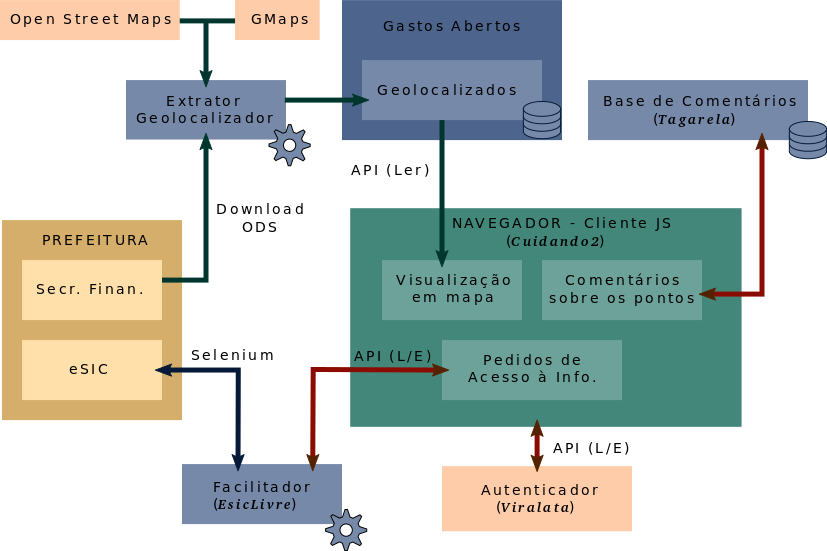
\includegraphics{cuidando2_arq2-827px.png}

As setas avermelhadas indicam conexões em que as escritas provavelmente
necessitarão de um
\href{https://github.com/okfn-brasil/viralata\#protocol}{token}.

A navegação HTML é de responsabilidade do \href{https://github.com/okfn-brasil/cuidando2}{Cuidando2}, implementado
atualmente em \href{https://cuidando.vc}{cuidando.vc}, que através de
\href{https://en.wikipedia.org/wiki/Ajax\_(programming)}{Ajax} faz a
comunicação com cada módulo, nos respectivos
\href{http://www.w3.org/TR/wsdl20/\#Endpoint}{endpoints}:

\begin{tabulary}{\linewidth}{|L|L|L|L|}
\hline
\textsf{\relax 
Função
} & \textsf{\relax 
Responsabilidade
} & \textsf{\relax 
\textbf{Endpoint} em uso
} & \textsf{\relax 
Notas
}\\
\hline
Geolocalização
 & 
\emph{Gastos Abertos}
 & 
\href{https://site-cuidando.rhcloud.com/dados/api/v1}{site-cuidando.rhcloud.com/dados/api/v1}
 & 
leitura das coordenadas
\\
\hline
Dados de execução orçamentária
 & 
\emph{Gastos Abertos}
 & 
\href{http://demo.gastosabertos.org}{demo.gastosabertos.org}
 & 
consulta à base de dados
\\
\hline
Autenticação dos usuários
 & 
\href{https://github.com/okfn-brasil/viralata}{Vira-Lata}
 & 
\href{https://viralata-cuidando.rhcloud.com}{viralata-cuidando.rhcloud.com}
 & 
token de acesso, leitura/escrita
\\
\hline
Comentários dos usuários
 & 
\href{https://github.com/okfn-brasil/tagarela}{Tagarela}
 & 
\href{https://tagarela-cuidando.rhcloud.com}{tagarela-cuidando.rhcloud.com}
 & 
leitura/escrita dos textos
\\
\hline
Interface com eSIC
 & 
\href{https://github.com/okfn-brasil/esiclivre}{EsicLivre}
 & 
\href{https://cuidando.vc/esiclivre}{cuidando.vc/esiclivre}
 & 
realização de pedidos de informação, leitura/escrita
\\
\hline\end{tabulary}


Cada um desses \emph{endpoints} apresenta também uma documentação mais
detalhada da API quando acessado diretamente do navegador,
exemplificando o uso de cada uma das operações
\href{https://en.wikipedia.org/wiki/Representational\_state\_transfer}{REST}
disponíveis no microserviço.


\chapter{Modos de operação e replicação}
\label{index:modos-de-operacao-e-replicacao}
Conforme a finalidade, o projeto pode ser copiado e adaptado, parcial ou
integralmente. O caso típico é a replicação para atuar com outros
municípios, mudando apenas o escopo de dados no Gastos Abertos e
adaptando-se o \emph{EsicLivre} para as peculiaridades do eSIC do município.

Uma outra forma comum de replicação é a integral, quando se deseja
instalar e testar localmente (o programador no seu computador) para
entender melhor o funcionamento do software como um todo, ou para
realizar (através de \emph{fork}) adaptações maiores.


\section{Replicando apenas o site}
\label{index:replicando-apenas-o-site}
Na ausência de dados da cidade, operaria em modo ``somente leitura''. Util
para designers e trabalhos restritos ao site.

Uma versão compacta das instruções a seguir, é oferecida também em \href{https://github.com/okfn-brasil/cuidando2-doc/blob/master/src/site.sh}{site.sh}.


\subsection{Escolhas e convenções}
\label{install-site::doc}\label{install-site:escolhas-e-convencoes}
O projeto pode rodar nas mais diversas plataformas com um mínimo de
adaptações. A título de homologação, todavia, apenas um ambiente foi
apreciado.

Para a obtenção de uma documentação mais clara e limpa foi adotada
\href{https://en.wikipedia.org/wiki/Convention\_over\_configuration}{convention over
configuration},
ou seja, não serão comentadas todas as possibilidades de configuração,
pressupomos certas convenções, e ficaria a cargo do usuário ou de uma
documentação secundária qualquer desvio da convenção adotada. Padrões de
referência:
\begin{itemize}
\item {} 
Sistema Operacional: Arch Linux 64 bits.

\item {} 
Navegadores homologados: Firefox 42+, Chorme 46+.

\end{itemize}


\subsection{Conferir ambiente}
\label{install-site:conferir-ambiente}
Será entendido como ``ambiente'' do servidor do projeto,
\begin{itemize}
\item {} 
Linux \textbf{Ubuntu 14.04+ LTS}: pode ser mais atualizado, mas são
pressupostas restrições do LTS nos exemplos de atualização. Conferir
com \code{lsb\_release -a} (resultará ex. 14.04.3).

\item {} 
\textbf{Git 1.9+}: \code{git -{-}version} (ex. 1.9.1).

\item {} 
Server-side \textbf{Javascript engine V8, v4.6+}:
\code{node -p process.versions.v8} (ex. 4.6.85)

\item {} 
\textbf{NodeJS v5.2+}: \code{nodejs -{-}version}(ex. v5.2.0)

\item {} 
\textbf{npm 3.5+} (do NodeJS): \code{npm -v} (ex. 3.5.2) ou \code{npm version},
que mostra também o nodejs e o v8.

\end{itemize}


\subsubsection{Atualizar o ambiente}
\label{install-site:atualizar-o-ambiente}
As versões mínimas indicadas de \emph{NodeJS} e \code{npm} precisam ser
respeitadas. Na sua instalação default o UBUNTU 14 LTS, todavia, não
oferece versões atualizadas, nem mesmo após o tradicional
\code{apt-get install}. O procedimento mais simples e correto para instalar
é o seguinte:

\begin{Verbatim}[commandchars=\\\{\}]
curl \PYGZhy{}sL https://deb.nodesource.com/setup\PYGZus{}5.x \textbar{} sudo \PYGZhy{}E bash \PYGZhy{}
sudo apt\PYGZhy{}get install \PYGZhy{}y nodejs
\end{Verbatim}

que já é suficiente para ambos, \emph{NodeJS} e \code{npm}. Confira as versões
com \code{npm -v} e \code{nodejs -{-}version}. O V8 em geral já se encontra
atualizado, mas vale conferir com \code{nodejs -p process.versions.v8}.

Nota: o \code{npm} vem com o \code{nodejs}, \emph{evite} o \code{apt-get install npm}
pois pode aparentar erro ou gerar versão muito antiga. Para garantir a
atualização do \code{npm} use ele mesmo,

\begin{Verbatim}[commandchars=\\\{\}]
sudo npm install npm \PYGZhy{}g
\end{Verbatim}


\subsection{Clonar e instalar o projeto}
\label{install-site:clonar-e-instalar-o-projeto}
\begin{Verbatim}[commandchars=\\\{\}]
git clone https://github.com/okfn\PYGZhy{}brasil/cuidando2.git
cd cuidando2
\end{Verbatim}

Em seguida verifique as configurações de \code{configs/config.js}. O caso
típico é mudar apenas o domínio para o local de teste,

\begin{Verbatim}[commandchars=\\\{\}]
nano configs/config.js
  ...
  const \PYGZus{}domain = \PYGZsq{}http://localhost:\PYGZsq{}
  ...
\end{Verbatim}

Caso não vá apenas simular o site, ou apenas reusar os microserviços de
São Paulo, há que se configurar mais parâmetros. Feito isso, roda a
instalação:

\begin{Verbatim}[commandchars=\\\{\}]
npm i
\end{Verbatim}

O ultimo comando vai um barra de progresso... Sinal que está indo tudo
bem.


\subsection{Rodar}
\label{install-site:rodar}
Para rodar o site:

\begin{Verbatim}[commandchars=\\\{\}]
npm run dev
\end{Verbatim}

Depois acesse \code{localhost:5001} em um navegador. Se quiser que o código
atualize automaticamente conforme editar os arquivos, acesse
\code{localhost:5001/webpack-dev-server/}.

(disponível também em \href{https://github.com/okfn-brasil/cuidando2-doc/blob/master/install-services.md}{install-site.md}).


\section{Replicando serviços e preparo dos dados}
\label{index:replicando-servicos-e-preparo-dos-dados}
Para reproduzir os microserviços, deve-se reproduzir também as bases de
dados.

As instruções para replicação do \emph{software} estão em
\href{https://github.com/okfn-brasil/cuidando2-doc/blob/master/install-services.md}{install-services.md}. A preparação dos dados
pode ser realizada de três modos:
\begin{itemize}
\item {} 
\emph{sandbox}: base de dados mínima com dados de teste.

\item {} 
\emph{referência}: dados da base em operação, em um site Cuidando já
implantado.

\item {} 
\emph{novo}: construir uma base de dados nova (por exemplo para um novo
município). A metodologia e dicas encontram-se descritas \href{https://pt.wikiversity.org/wiki/Projeto\_Cuidando\_do\_Meu\_Bairro/Novos\_dados}{nesta
Wiki}.

\end{itemize}


\section{Replicação completa}
\label{index:replicacao-completa}
Para replicar ambos, o site e os serviços, um script mais consido também
é oferecido: \href{https://github.com/okfn-brasil/cuidando2-doc/blob/master/src/full.sh}{src/full.sh}.


\chapter{CRÉDITOS E LICENÇAS}
\label{index:creditos-e-licencas}
A presente documentação e todos os scripts \href{https://github.com/okfn-brasil/cuidando2-doc}{deste módulo de
documentação} estão
licenceados sob \href{http://creativecommons.org/licenses/by/4.0/}{CC-BY 4.0}.

O Cuidando2 é um projeto realizado por várias mãos,
\begin{itemize}
\item {} 
Alexandre Evangelista de Souza Júnior
(\href{https://github.com/alexandre}{@alexandre})

\item {} 
Andrés M. R. Martano (\href{https://github.com/andresmrm}{@andresmrm})

\item {} 
Gisele S. Craveiro (coordenação),

\item {} 
Jutta Machado Schimdt

\item {} 
Solaine Lima

\item {} 
... e todos os parceiros e beta-testers, que  auxiliaram com sugestoes criativas e construtivas

\end{itemize}

com apoio de,
\begin{itemize}
\item {} 
\href{http://colab.each.usp.br/}{COLAB-USP}

\item {} 
\href{http://br.okfn.org/}{OKBR}

\item {} 
? (financeamento)

\end{itemize}

e disperso por alguns módulos, listados a seguir com indicação das
respectivas licenças e equipes:
\begin{itemize}
\item {} 
\href{https://github.com/okfn-brasil/cuidando2.git}{Site Cuidando do
Município}: licença \href{https://github.com/okfn-brasil/cuidando2/blob/master/LICENSE.txt}{AGPLv3}.

\item {} 
\emph{equipe}: Gisele (coordenação), Andrés (software), Solaine (design).

\item {} 
\href{https://github.com/okfn-brasil/cuidando2/graphs/contributors}{Software}:
@andresmrm e @LuizArmesto

\item {} 
\href{https://github.com/okfn-brasil/gastos\_abertos}{Gastos Abertos}:
licença \href{https://github.com/okfn-brasil/gastos\_abertos/blob/master/LICENSE}{AGPLv3}
em nome de \href{http://br.okfn.org/}{OKBR}/\href{http://wiki.okfn.org/Open\_Knowledge\_Brasil/Gastos\_Abertos}{Projeto Gastos
Abertos}.

\item {} 
\href{https://github.com/okfn-brasil/gastos\_abertos/commits/master/data}{*Dados*}:
@aivuk, @andresmrm.

\item {} 
\href{https://github.com/okfn-brasil/gastos\_abertos/graphs/contributors}{*Software*}:
@andresmrm , @aivuk, @LuizArmesto, @waffle-iron, @carlosandrade,
@lpirola.

\item {} 
Demais
\href{https://en.wikipedia.org/wiki/Microservices}{microserviços} e
módulos de apoio:

\item {} 
\href{https://github.com/okfn-brasil/esiclivre}{eSIC Livre}: licença \href{https://github.com/okfn-brasil/esiclivre/blob/master/LICENSE.txt}{AGPLv3}.
\begin{itemize}
\item {} 
\emph{equipe}: @alexandre e @andresmrm

\end{itemize}

\item {} 
\href{https://github.com/okfn-brasil/tagarela}{Tagarela}: licença \href{https://github.com/okfn-brasil/tagarela/blob/master/LICENSE.txt}{AGPLv3},
software @andresmrm.

\item {} 
\href{https://github.com/okfn-brasil/viralata}{Viralata}: licença \href{https://github.com/okfn-brasil/viralata/blob/master/LICENSE.txt}{AGPLv3},
software @andresmrm.

\item {} 
\href{https://github.com/okfn-brasil/viratoken}{Viratoken}: licença \href{https://github.com/okfn-brasil/viratoken/blob/master/LICENSE.txt}{AGPLv3},
software @andresmrm.

\end{itemize}


\chapter{Indices and tables}
\label{index:indices-and-tables}\begin{itemize}
\item {} 
\DUspan{xref,std,std-ref}{genindex}

\item {} 
\DUspan{xref,std,std-ref}{modindex}

\item {} 
\DUspan{xref,std,std-ref}{search}

\end{itemize}



\renewcommand{\indexname}{Índice}
\printindex
\end{document}
